% Figure 1
\ffigbox[\FBwidth]{
\label{Fig:td2ex9}
}{
    \fbox{
        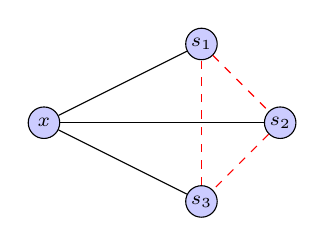
\begin{tikzpicture}[scale=1, every node/.style={circle, draw, fill=blue!20, inner sep=1pt, font=\scriptsize, minimum size=4mm}]
            \node (x) at (0, 1) {\(x\)};

            \node (s1) at (2, 2) {\(s_1\)};
            \node (s2) at (3, 1) {\(s_2\)};
            \node (s3) at (2, 0) {\(s_3\)};

            \draw (x) -- (s1);
            \draw (x) -- (s2);
            \draw (x) -- (s3);

            \draw[red, dashed] (s1) -- (s2);
            \draw[red, dashed] (s2) -- (s3);
            \draw[red, dashed] (s3) -- (s1);
        \end{tikzpicture}
    }
}